%\documentclass[12pt]{article}
%\usepackage{beamerarticle}

\documentclass[german]{beamer}

\usepackage[ngerman]{babel}
\usepackage[utf8]{inputenc}
\usepackage{amssymb}
\usepackage{pgfpages}
\usepackage{dsfont} 
\usepackage{bm}

\let\oldframe\frame
\renewcommand\frame[1][allowframebreaks]{\oldframe[#1]} % allowframebreaks als Standard

\mode<article>{\setbeamertemplate{frametitle}{}} % keine Frametitles im Artikel
  
\setbeamertemplate{note page}[plain]
\mode<presentation>{
\setbeameroption{show notes on second screen=left}
\AtBeginNote{\insertslideintonotes{0.5}\par}
\usetheme{Montpellier}
\beamertemplatenavigationsymbolsempty
} %end mode presentation

\setbeamertemplate{theorems}[ams style]
\setbeamertemplate{enumerate items}[default]
\setbeamertemplate{frametitle continuation}{} % Keine Nummerierung bei automatischem Umbruch

\setbeamertemplate{footline}{\hspace*{.2cm}\tiny \inserttitle \hfill \insertframenumber/\inserttotalframenumber \hspace*{.2cm}}

\newcommand{\mX}{{\bf X}}
\newcommand{\mx}{{\bf x}}
\newcommand{\mY}{{\bf Y}}
\newcommand{\my}{{\bf y}}

\title{Angewandte Bayes-Statistik}
\author{Volker Schmid}
\institute{LMU, Institut f\"ur Statistik}
\date{Sommersemester 2017}

\newtheorem{Bsp}{Beispiel}
\newtheorem{Def}{Definition}
\newtheorem{Stz}{Satz}

\numberwithin{Bsp}{section}
\numberwithin{Def}{section}
\numberwithin{Stz}{section}

\begin{document}
\mode<article>{
\begin{titlepage}
\begin{center}
\includegraphics{../pics/siegel}\\[1cm]    
\LARGE \textbf{Einführung in die Bayes-Statistik}\\[5mm]

\Large  Volker Schmid, Clara Happ \\
        27.--30. März 2017\\[1cm]

        Institut f{\"u}r Statistik \\
        Ludwig--Maximilians--Universit{\"a}t M{\"u}nchen\\[1cm]
        
\vfill
\end{center}

\end{titlepage}
\small
\tableofcontents
\newpage
}

\mode<presentation>{
\newcommand{\paragraph}[1]{} % ignoriere paragraph
\begin{frame}
  \titlepage
\end{frame}
}
\section{Einleitung}
\subsection{Thomas Bayes}
\begin{frame}{Thomas Bayes}
\begin{center}
\only<1->{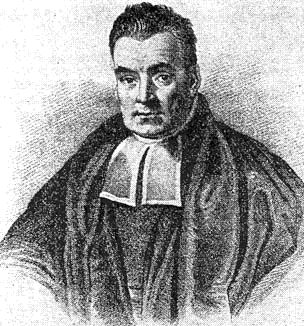
\includegraphics[width=150px]{../pics/Thomas_Bayes.png}}
\note{Einziges Bild, vermutlich nicht authentisch}

\end{center}
\end{frame}

\begin{frame}{Thomas Bayes}
\begin{center}
{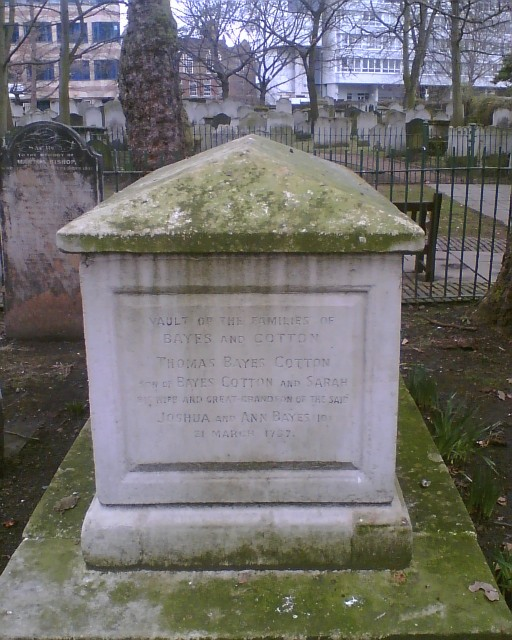
\includegraphics[width=120px]{../pics/Image028.jpg}}
\note{
\begin{itemize}
\item Priester (wie der Vater) und Mathematiker
\item lebte in Tunbridge Wells (s\"ud\"ostlich von London)
\item beeinflusst von Abraham de Moivre (frz. Mathematiker, unter anderem Thema Gl\"ucksspiel, Satz von de Moivre-Laplace = Grenzwertsatz f\"ur Bionomialverteilung)
\item Drei bekannte Werke: G\"ottliche Barmherzigkeit, oder ein Versuch zu beweisen, dass das Ziel der g\"ottlichen F\"ursorge und Gewalt das Gl\"uck seiner Gesch\"opfe ist; Eine Einfh\"urng in die Lehre der Analysis und eine Verteidigung der Mathematiker gegen die Einwände des Autor von ``The Analyst'' (George Berkeley, anonym erschienen)
\end{itemize}
}
\end{center}
\end{frame}

\begin{frame}{Kurze Geschichtlicher Überblick}
\begin{itemize}
\item Mitte 18. Jahrhundert: Bayes entwickelt die Bayes-Formel
\item Anfang 19. Jahrhundert: Pierre-Simon Laplace entwickelt die Bayes-Formel, prägt den Begriff ''Inverse Wahrscheinlichkeit''
\item Anfang 20. Jahrhundert: Ronald Fisher entwickelt den Frequentismus, Maximum-Likelihood-Schätzer, prägt den Begriff ''Bayes-Statistik''
\item Ende des 20. Jahrhunderts: Bayes-Verfahren werden wieder aktuell, komplexe Modelle dank Computer möglich
\end{itemize}
\footnotesize Literatur:  Stephen E. Fienberg: When Did Bayesian Inference Become
''Bayesian''? Bayesian Analysis (2006) 1(1), pp. 1–40.
\end{frame}

\subsection{Bayes und die Billardkugeln}

\begin{frame}{Beispiel nach Bayes}
\begin{Bsp}[An Essay towards solving a Problem in the Doctrine of Chance (1763)]
\label{bsp:kugelnachbayes}
Eine weiße Billiardkugel wird auf eine Gerade der Länge 1 gerollt. Die Wahrscheinlichkeit dafür, dass sie an einem Punkt $\pi$ zu liegen kommt, ist konstant für alle $\pi \in [0,1]$. Eine rote Kugel wird unter den selben Bedinungen $n$-mal gerollt. Sei $x$ die Zahl der Versuche, in denen die rote Kugel links von der ersten Kugel, also links von $\pi$ zu liegen kommt.

Welche Information über $\pi$ erhalten wir aus der Beobachtung $x$?
\end{Bsp}
%\end{frame}

%\begin{frame}{Billardkugeln}
Sei die weiße Kugel bereits gerollt und liege auf dem Punkt $\pi$. Die rote Kugel gerollt. Dann ist die Wahrscheinlichkeit, dass die rote Kugel links von der weißen zu liegen kommt gleich $\pi$. Rollen wir $n$-mal, so handelt es sich um ein Binomialexperiment mit Erfolgswahrscheinlichkeit $\pi$. Gegeben $\Pi=\pi$ ist also:
\[
P(X=x|\Pi=\pi)=f(x|\pi)={{n}\choose{x}}\pi^x(1-\pi)^{n-x}.
\]

Um nun mit dem Satz von Bayes eine Aussage über $pi$ gegeben $x$ zu machen, brauchen wir $f(\pi)$. Was wissen wir  über $\pi$ vor der Beobachtung?
\end{frame}

\begin{frame}{Priori und Posteriori}
Annahme: Vor der Beobachtung, lateinisch \textit{a priori}, wissen wir nichts über $\pi$. Wir folgen dem Prinzip von unzureichenden Grund und nehmen $\pi \sim U[0,1]$. 

Dann erhalten wir nach der Beobachtung, lateinisch \textit{a posteriori}, mit dem Satz von Bayes
\begin{eqnarray}
f(\pi|x)&=&\frac{f(x|\pi)f(\pi)}{\int{f(x|\tilde\pi)f(\tilde\pi)d\tilde\pi}} = \frac{{{n}\choose{x}}\pi^x(1-\pi)^{n-x}\cdot 1}{f(x)} \nonumber\\
&=& C(x) \cdot \pi^x (1-\pi)^{n-x} = C(x) \cdot \pi^{(x+1)-1} (1-\pi)^{(n-x+1)-1} \label{eq:postbilliard}
\end{eqnarray}
Dabei ist $C(x)$ eine Konstante bezüglich $\pi$ (hängt nicht von $\pi$, nur von $x$ ab). (\ref{eq:postbilliard}) sieht bis auf die Konstante aus wie die Dichte der Beta$(x+1,n-x+1)$-Verteilung. Wir sagen: $\pi^{(x+1)-1} \pi^{(n-x+1)-1}$ ist der ''Kern'' der Beta-Verteilung.
\end{frame}

\begin{frame}{}
\begin{itemize}
\item Wir haben Vorwissen über die Wahrscheinlichkeit $\pi$ in Form einer \textbf{Priori-Verteilung} bzw. Priori -Dichte formuliert.
\item Nach der Beobachtung $x$ wissen wir mehr über $\pi$; wir haben die \textbf{Posteriori-Verteilung} bzw. Posteriori-Dichte erhalten.
\item Bayes-Prinzip: Alle Schlüsse werden aus der Posteriori-Verteilung gezogen.
\item Zur Berechnung der Posteriori brauchen wir zudem das Beobachtungsmodell bzw. \textbf{Datendichte} $f(x|\pi)$ (auch als Likelihood bezeichnet)
\item und die \textbf{Normalisierungskonstante} (auch marginale Likelihood), die wir hier nicht explizit berechnen mussten.
 \end{itemize}
\end{frame}

\begin{frame}{Priori und Posteriori}
\mode<article>{
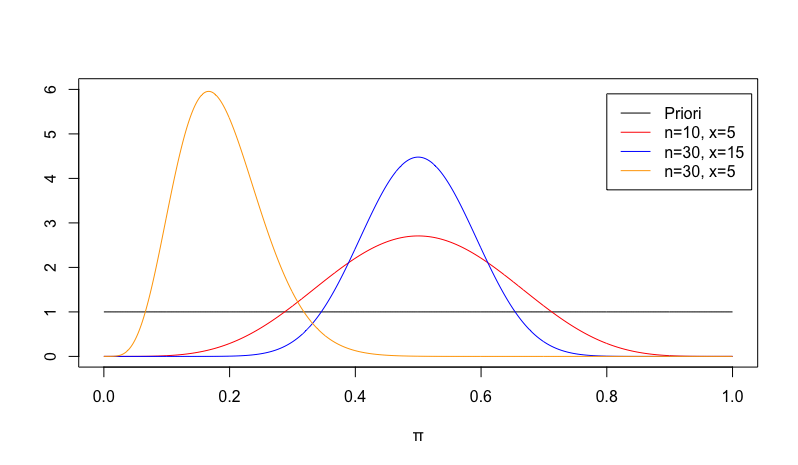
\includegraphics[scale=.5]{../pics/betapost.png}
}
\mode<presentation>{
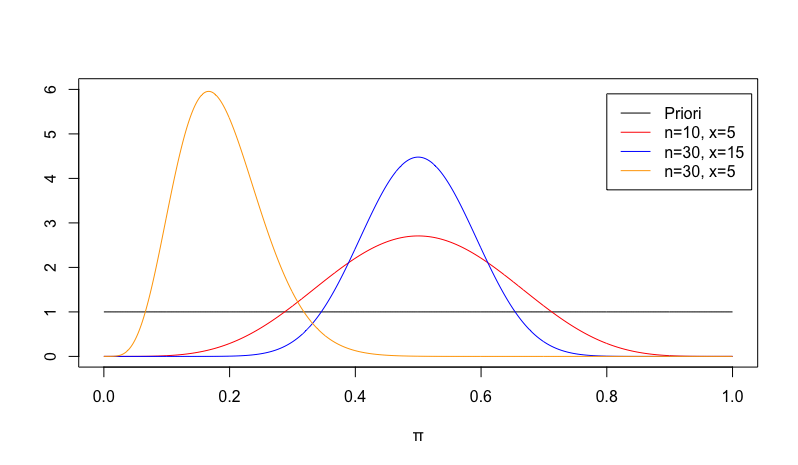
\includegraphics[scale=.4]{../pics/betapost.png}
}
\end{frame}


\subsection{Bayesianische Inferenz}
\begin{frame}{Bayesianische Inferenz}
\begin{itemize}
\item Wir beobachten $n$ Daten $x_i$, die aus einem Zufallsprozess entstanden sind
\item \textbf{Annahme}: $x_i$ ist die Realisierung einer Zufallsvariable $X_i$
\item \textbf{Annahme}: $X_i$ hat Verteilung $F$ mit Dichte $f(x)$
\note{Wir brauchen die Dichte! Wie bei Likelihood-Inferenz!\\
Abweichungen davon möglich (z.B. Maximum Entropy Methoden, Quasi-Likelihood)\\
Dichte kommt aus dem (statistischen) Modell}
\item \textbf{Parametrische Annahme}: Die Dichte ist bekannt bis auf einen Parameter $\theta$: $f(x|\theta)$
\item $\theta$ ist unbekannt und die Information über $\theta$ lässt sich in Form einer Wahrscheinlichkeitsverteilung mit Dichte darstellen
\item Vor der Beobachtung (\textit{a priori}) ist unsere Information $p(\theta)$ 
\item Durch Beobachtung erhalten wir mehr Information, ausgedrückt durch die \textit{a posteriori}-Verteilung $\theta|x$
\item Sowohl $x$ als auch $\theta$ können mehrdimensional sein!
\end{itemize}
\end{frame}

\begin{frame}{Aufgaben in der Bayesianischen Inferenz}
\begin{itemize}
\item Festlegung des statistischen Modells für $x$, Datendichte (Likelihood) $f(x|\theta)$ 
\note{Einfachstichprobe, identisch, iid., Regressionsmodell?\\}
\item Festlegung des \textit{a priori}-Wissens über $\theta$, Priori-Dichte $p(\theta)$  
\note{Konjugierte Priori, nicht-informative Priori, subjektive Priori, imprompere Priori\\}
\item Berechnung der Posteriori $p(\theta|x)$ (insbesondere Normalisierungskonstante)
\note{Analytisch, Approximation, Monte-Carlo}
\end{itemize}
\end{frame}

\begin{frame}{Bayes-Prinzip}
\begin{itemize}
\item Die Dichte der Posteriori-Verteilung erhalten wir über die Bayes-Formel
\end{itemize}
\begin{center}
\framebox{
\LARGE
$f(\theta|x) = \frac{f(x|\theta) \cdot f(\theta)}{\int f(x|\tilde\theta) f(\tilde\theta) d\tilde\theta}$
}
\end{center}
\begin{itemize}
\item Bayes-Prinzip: Alle Schlüsse werden \textbf{nur} aus der Posteriori-Verteilung gezogen
\end{itemize}
\end{frame}

\begin{frame}{Punktschätzer}
Billiard-Kugel-Beispiel: sei $n=30$ und $x=5$. Wie lautet dann unser Schätzer für $\pi$? 
\begin{itemize}
\item Posteriori-Erwartungswert: Nach Beobachtung von $x$, welchen Wert erwarten wir für $\pi$?\\
$$ E(\pi)=\frac{x+1}{n+1}=\frac{6}{31}\approx 0.194$$
\item Posteriori-Modus: Welcher Wert von $\pi$ maximiert die Posteriori?
$$ \hat{\pi}_{\text{MAP}}=\frac{x}{n}=\frac{5}{30} \approx 0.167$$
\item Posteriori-Median: Welcher Wert hat die mittlere Wahrscheinlichkeit?
$$ \hat{\pi}_{\text{med}}\approx 0.181$$
\end{itemize}
\end{frame}

\begin{frame}{Kredibilitätsintervall}
Aus der Posteriori-Verteilung lässt sich ein Intervall $[\theta_u, \theta_o]$ bestimmen, das den Parameter $\theta$ mit Wahrscheinlichkeit $(1-\alpha)$ enthält.
\begin{Def}
Ein Intervall $I = [\theta_u, \theta_o]$, für das gilt
\[ 
\int_{\theta_u}^{\theta_o} p(\theta|x)d\theta = 1-\alpha
\]
nennt man $(1-\alpha)$-\textbf{Kredibilitätsintervall}.
\end{Def}
\end{frame}

\begin{frame}{HPD-Intervall}
Kredibilitätsintervalle sind nicht eindeutig. 
\begin{Def}
Ein $(1-\alpha)$-Kredibilitätsintervall $H$ heisst \textbf{Highest Posteriori Density Interval (HPD-Intervall)}, wenn für alle $\theta \in H$ und alle $\theta^* \not\in H$ gilt:
\[ p(\theta|x) \geq p(\theta^*|x) \]
\end{Def}
\end{frame}

\begin{frame}{}
\mode<presentation>{
\begin{Bsp}[Kredibilitätsintervalle Betabinomialmodell]
\centering
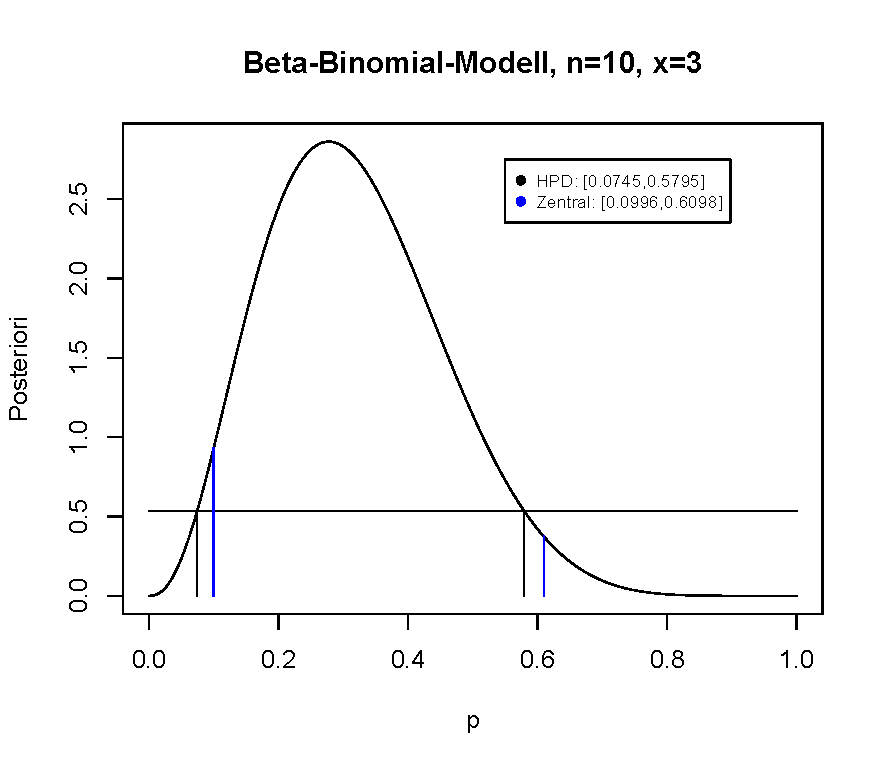
\includegraphics[scale=.5]{../pics/KI-Betabinomial.pdf}
\end{Bsp}
}
\mode<article>{
\begin{Bsp}[Kredibilitätsintervalle Betabinomialmodell]
\end{Bsp}
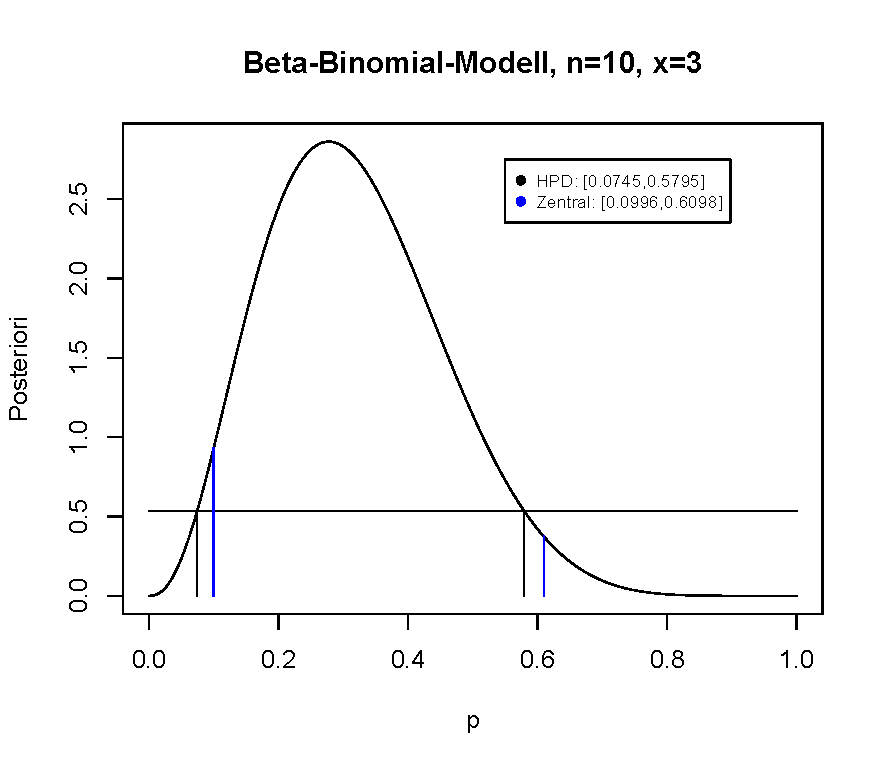
\includegraphics[scale=.7]{../pics/KI-Betabinomial.pdf}
}
\note{Länge der Intervalle: 0.5102 und 0.505}
\end{frame}

\begin{frame}{Prädiktive Posterioriverteilung}
\begin{Def}
Die Dichte der \textbf{Prädiktiven Posteriori-Verteilung} lautet
\[
p(x_Z|x)=\int_\Theta p(x_Z,\theta|x) d\theta = \int p(x_Z|\theta)p(\theta|x) d\theta 
\]
\end{Def}
Die prädiktive Posteriori-Verteilung ermöglicht die Prognose von $x$ zum Zeitpunkt $Z$. Es gilt:
\begin{eqnarray*}
E(x_Z|x) &=& E(E(x_Z|\theta,x))\\
Var(x_Z|x)&=& E(Var(x_Z|\theta,x))+Var(E(x_Z|\theta,x))
\end{eqnarray*}
\end{frame}

\begin{frame}{Aufgaben in der Bayesianischen Inferenz}
``Bayes-Prinzip: Alle Schlüsse werden \textbf{nur} aus der Posteriori-Verteilung gezogen'' -- Was machen wir nun mit der Posteriori?
\begin{itemize}
\item Grundsätzlich: Komplette Posteriori wichtig (Darstellung bei hochdimensionalem Parameter $\theta$ aber schwierig)
\item Punktschätzer (Posterior-Erwartungswert, Maximum-a-Posteriori-Schätzer, Posteriori-Modus)
\item Intervallschätzer
\item Testen
\item Modellvergleich (d.h. verschiedene Annahmen für $f(x)$!)
\item Prädiktion
\end{itemize}
\end{frame}

\subsection{Bayesianische Modellierung}
\subsubsection{Normalverteilungsmodel}
\begin{frame}{Normalverteilung}
Gegeben seien $n$ unabhängig normalverteilte Beobachtungen
$$ 
X_i \sim  N(\mu,\sigma^2), i=1,\ldots,n.
$$ 
Die gemeinsame Datendichte lautet
\begin{eqnarray*}
f(x|\theta) &=& \prod\left(f(x_i|\theta)\right) \\
&=& \left(\frac{1}{\sigma\sqrt(2\pi)}\right)^n \exp\left(-\frac{1}{2\sigma^2}\sum_{i=1}^n (x_i-\mu)^2\right)
\end{eqnarray*}
\end{frame}

\paragraph{$\sigma^2$ bekannt}
\begin{frame}{Normalverteilungsmodell für $\sigma^2$ bekannt}
Konjugierte Priori $\mu\sim N(\mu_0,\sigma_0^2)$. Damit ist die Posteriori
\begin{eqnarray*}
\mu|(x_1,\ldots,x_n) &\sim &N(m/s,1/s)\\
m&=&\frac{\mu_0}{\sigma_0^2} + \frac{\sum_{i=1}^n x_i}{\sigma^2}\\
s &=& \frac{1}{\sigma_0^2} + \frac{n}{\sigma^2}
\end{eqnarray*}

Jeffreys Priori: $p(\mu)\propto$ const. entspricht $\sigma^2_0\to\infty$.
\end{frame}

\paragraph{$\mu$ bekannt}
\begin{frame}{Normalverteilung für $\mu$ bekannt}
Konjugierte Priori: $\sigma^2\sim IG(a,b)$ führt zur Posteriori
\[
\sigma^2|(x_1,\ldots,x_n) \sim IG\left(a+n/2, b+0.5\sum_{i=1}^n{(x_i-\mu)^2}\right)
\]

Jeffreys Priori $p(\sigma^2)\propto\sigma^{-1}$ entspricht ''IG(0,0)''.
\end{frame}

\begin{frame}{Normalverteilung für $\mu$ bekannt}
Alternativ lässt sich die Inferenz für die Präzision gleich Inverse der Varianz betreiben:
$$ \tau=\sigma^{-2}. $$
Die konjugierte Priori ist dann die Gamma-Verteilung
\[
p(\tau) = \frac{b^a}{\Gamma(a)}\tau^{a-1}\exp{-b\tau}.
\]
Die Posteriori lautet
$$
p(\tau|x)\propto \tau^{n/2}\exp\left(-\tau/2\sum_{i=1}^n(x-\mu)^2\right)\cdot\tau^{a-1}\exp(-b\tau),
$$
ist also die Ga($a+n/2, b+0.5\sum_{i=1}^n{(x_i-\mu)^2}$)-Verteilung.
\end{frame}

\paragraph{Zwei unbekannte Parameter}
\begin{frame}{Normalverteilungsmodell mit zwei unbekannten Parametern}
Bei jeweils einem unbekanntem Parameter und unter Benutzung der konjugierten Verteilung kennen wir die Posteriori vollständig. Im Folgenden seien beide Parameter ($\mu$ und $\tau$) unbekannt.

Wir wollen die selben Prioris wie oben benutzen und gehen von \textit{a priori}-Unabhängigkeit der Parameter aus:
$$ p(\mu,\tau)=p(\mu)\cdot p(\tau) $$

Die Posteriori lautet bis auf Konstanten:
\begin{eqnarray*}
p(\mu,\tau|x)&\propto& \exp\left(-\tau_0/2 (\mu-\mu_0)^2\right)\\
&&\cdot\tau^{n/2}\exp\left(-\tau/2\sum_{i=1}^n(x-\mu)^2\right)\cdot\tau^{a-1}\exp(-b\tau)
\end{eqnarray*}
\note{Dabei handelt es sich nicht um eine bekannte zweiparametrische Verteilung.}
\end{frame}


\begin{frame}{Bedingte Posteriori}
Wir betrachten die bedingte Posteriori eines Parameters, z.B. $p(\mu|\tau,x)$. Nach der Definition der bedingten Dichte gilt
\[
p(\mu|\tau,x)=\frac{p(\mu,\tau|x)}{p(\tau|x)}\propto p(\mu,\tau|x)
\]
Hier also: Die bedingte Posteriori-Dichte von $\mu$ gegeben $\tau$ ist die Normalverteilung. Das ergibt sich automatisch aus dem Normalverteilungsmodell mit bekannter Varianz!

Die bedingte Posteriori hilft uns aber nicht weiter, weil wir den Parameter $\tau$ nicht kennen.
\end{frame}

\begin{frame}{Vollständig bedingte Posteriori}
\begin{Def}(Vollständig bedingte Posterior)
Sei $\bf{\theta}=(\theta_1,\ldots\theta_p)$. Als vollständig bedingte Posteriori (''full conditional posterior'') bezeichnen wir die Verteilung eines Parameters $\theta_i$ gegeben allen anderen Parametern $\theta_{-i}$ und den Daten $x$. Es gilt:
$$
 p(\theta_i|\theta_{-i},x)\propto p(\bf{\theta}|x).
$$
\end{Def}

\begin{Def}(Semikonjugierte Priori)
Eine Familie $\mathcal{F}$ von Verteilungen auf $\Theta$ heißt \textbf{semikonjugiert} wenn für jede Priori $p(\theta)$ auf $\mathcal{F}$ die vollständig bedingte Posteriori $p(\theta_i|\theta_{-i},x)$ ebenfalls zu $\mathcal{F}$ gehört. 
\end{Def}
\end{frame}

\begin{frame}{Marginale Posteriori}
Wir betrachten die marginale Posteriori eine Parameters, also z.B. $p(\tau|x)$. Diese erhalten wir durch marginalisieren der gemeinsamen Posteriori
$$ 
p(\tau|x)=\int p(\mu,\tau|x) d\mu. 
$$
Alternativ kann man folgende Formel ausnutzen
$$
p(\tau|x)=\frac{p(\mu,\tau|x)}{p(\mu|\tau,x)}
$$

Interessiert uns in mehrparametrischen Modellen nur ein Parameter, so ziehen wir die Schlüsse aus der marginalen Posteriori (\textit{"Model averaging"}).
\end{frame}


\subsubsection{Regression}

\paragraph{Lineare Regression}
\begin{frame}{Lineare Regression}
Übliches Lineares Regressionsmodell:
\begin{eqnarray*}
y_i&=&\alpha+\beta x_i+\epsilon_i\\
{\rm E}(\epsilon)&=&0\\
{\rm Var}(\epsilon)&=&\sigma^2\\
{\rm Cov}(\epsilon_i,\epsilon_j)&=&0\\
\end{eqnarray*}
\end{frame}

\paragraph{Bayesianisches lineares Regressionsmodell}
\begin{frame}{Bayesianisches lineares Regressionsmodell}
\begin{eqnarray*}
y_i &\sim & {\rm N}(\alpha+\beta x_i,\sigma^2)\\
\alpha&\sim&{\rm N}(m_\alpha,v_\alpha^2)\\
\beta &\sim&{\rm N}(m_\beta,v_\beta^2)
\end{eqnarray*}
Bei festem $\sigma^2$ sind dies die konjugierten Prioris.
Wir kennen allerdings $\sigma^2$ in der Regel nicht. Wir nehmen zusätzlich an:
\[
\sigma^2 \sim IG(a,b)
\]
\note{Vorrechnen: gesamte Posteriori, marginale Posteriori}
\end{frame}

\paragraph{Generalisierte Lineare Regression}
\begin{frame}{Bayesianisches generalisiertes lineares Regressionsmodell}
Das Modell lässt sich relativ einfach auf beliebige Verteilungen verallgemeinern, z.B. ein Poisson-Modell
\begin{eqnarray*}
y_i &\sim& Po(\lambda_i)\\
\log(\lambda_i) &=& \alpha+\beta x_i\\
\alpha&\sim&{\rm N}(m_\alpha,v_\alpha^2)\\
\beta &\sim&{\rm N}(m_\beta,v_\beta^2)
\end{eqnarray*}
Die (vollständig bedingten) Posterioris sind jedoch keine Standardverteilungen mehr.
\note{
$$ f(y_i|\lambda) = \frac{\lambda_i^{y_i}}{y_i!}\exp{-\lambda_i}$$
$$ \lambda_i=\exp(\alpha+\beta x_i) $$
}
\end{frame}

\paragraph{Multivariate Regression}
\begin{frame}{Multivariate Normal-Regression}
\begin{eqnarray}
y_i &\sim & {\rm N}(\mathbf{x}_i\boldsymbol\beta,\sigma^2)\\
\sigma^2&\sim&IG(a,b)\\
{\boldsymbol\beta} &\sim&{\rm N}(\mu_0,\boldsymbol\Lambda^{-1}_0)
\end{eqnarray}
\end{frame}
\begin{frame}{Posteriori}
\begin{eqnarray*}
p(\boldsymbol\beta,\sigma^{2}|\mathbf{y}) &\propto& f(\mathbf{y}|\boldsymbol\beta,\sigma^{2})p(\boldsymbol\beta)p(\sigma^{2})\\
&\propto&  (\sigma^{2})^{-n/2} \exp\left(-\frac{1}{2{\sigma}^{2}}(\mathbf{y}- \mathbf{X} \boldsymbol\beta)^{\rm T}(\mathbf{y}- \mathbf{X} \boldsymbol\beta)\right)\\
&\cdot&     |\boldsymbol\Lambda_0|^{1/2} \exp\left(-\frac{1}{2}(\boldsymbol\beta -\boldsymbol\mu_0)^{\rm T} \boldsymbol\Lambda_0 (\boldsymbol\beta - \boldsymbol\mu_0)\right)\\
&\cdot&  (\sigma^2)^{-(a_0+1)} \exp\left(-\frac{b_0}{{\sigma}^{2}}\right)
\end{eqnarray*}

$$ 
p(\beta|\sigma^2,\mathbf{y}) \propto \exp\left(-\frac{1}{2}\boldsymbol\beta^{\rm T}({\sigma}^{2}\mathbf{X}^{\rm T}
\mathbf{X}+\boldsymbol\Lambda_0)\boldsymbol\beta + (\sigma^2\mathbf{y}^{\rm T}\mathbf{X}+\boldsymbol
\mu_0^{\rm T}\boldsymbol \Lambda_0)\boldsymbol \beta)\right) 
$$
\end{frame}

\begin{frame}{Full conditionals}
Damit 
\begin{eqnarray}
\boldsymbol\beta|\sigma^2,\mathbf{y},\mathbf{x} &\sim& N(\boldsymbol\mu_n,\sigma^2\boldsymbol\Lambda_n^{-1})\\
\sigma^2|\boldsymbol\beta,\mathbf{y},\mathbf{x}&\sim& IG(a_n,b_n)\\
\boldsymbol\mu_n&=&(\sigma^2\mathbf{X}^{\rm T}\mathbf{X}+\boldsymbol\Lambda_0)^{-1} (\boldsymbol\Lambda_0\boldsymbol\mu_0+\sigma^2\mathbf{y}^{\rm T}\mathbf{X}\hat{\boldsymbol\beta})\\
\boldsymbol\Lambda_n&=&(\sigma^2\mathbf{X}^{\rm T}\mathbf{X}+\boldsymbol\Lambda_0) \\
a_n&=&a_0+\frac{n}{2}\\
b_n&=&b_0+\frac{1}{2}(\mathbf{y}^{\rm T}\mathbf{y}+\boldsymbol\mu_0^{\rm T}\boldsymbol\Lambda_0\boldsymbol\mu_0-\boldsymbol\mu_n^{\rm T}\boldsymbol\Lambda_n\boldsymbol\mu_n) 
\end{eqnarray}
\end{frame}

\begin{frame}{Random Walk Priori}
Über die Kovarianz- oder die Präzisionsmatrix lassen sich Korrelationen zwischen den Kovariableneffekten modellieren. Z.B. ein zeitlich geglätterer Trend.
\begin{Bsp}[Random Walk Priori]
Gegeben sei eine Zeitreihe $y_t$ mit $t=1,\ldots,T$. Wir wollen die Zeitreihe glätten. Sei $\mathbf{X}=\mathbf{I}_T$, dann ist obiges Modell gleich
$$y_t =\beta_t + \epsilon_t \text{ für }t=1,\ldots,T$$
Als Priori für $\beta$ nehmen wir einen ''Random Walk'':
\begin{eqnarray*}
\beta_1 &\sim &N(0,\tau_0^2)\\
\beta_t &\sim &N(\beta_{t-1},\tau^2)\\
\end{eqnarray*}
Der Parameter $\tau$ steuert die \textit{Glattheit} der Zeitreihe $\beta_t$.
\end{Bsp}
\end{frame}

\begin{frame}{Präzisionsmatrix}
Es lässt sich zeigen (mit $\tau_0\to \infty$): 
$$ \Lambda = \tau^{-2}\left(\begin{array}{ccccccc}
1 & -1 & 0 & \cdots & & & 0\\
-1 & 2 & -1 & 0 & \cdots & & 0\\
0 & -1 & 2 & -1 & 0 & \cdots & 0\\
\vdots & & & \ddots & \ddots& \ddots & \vdots \\
& &  \cdots & 0 & -1 & 2 & -1 \\
& & & \cdots & 0 & -1 & 1
\end{array}\right) $$
\end{frame}

\begin{frame}
\mode<article>{
\includegraphics[scale=.7]{../pics/globalwarming-rw.png}
}
\mode<presentation>{
\centering
\includegraphics[scale=.5]{../pics/globalwarming-rw.png}
}
\end{frame}

\subsubsection{Hierarchische Modellierung}
\begin{frame}{Hierarchische Bayesianische Modelle}
\begin{itemize}
\item[] Level 1: Datenmodell, Definition der Likelihood
\item[] Level 2: Priori-Modell der unbekannten Parameter
\item[] Level 3: (Hyper-)Prioris der Prioriparameter in Level 2
\end{itemize}
Kann an sich beliebig erweitert werden, i.d.R. reichen aber drei Level. Inferenz üblicherweise mit MCMC.
\end{frame}


\begin{frame}
\begin{Bsp}[Räumliches APC-Modell]
\label{bsp:raeumlichesapc}
Anzahl männliche Magenkrebstote in Westdeutschland
\begin{itemize}
\item Jahre 1976 - 1990
\item 13 Altersgruppen a 5 Jahre (15-19 bis 85-89)
\item Geburtskohorten von 1896-1975
\item 30 Regierungsbezirke
\end{itemize}
\end{Bsp}
\end{frame}

\begin{frame}{Hierarchisches Bayesianisches Modell: Level 1}
\begin{eqnarray}
y_{ijt} &\sim& \mbox{B}(n_{ijt},\pi_{ijt})\\
\mbox{logit}(\pi_{jtl}) &=& \xi_{jtl} \\ 
&=& \mu + \theta_j + \phi_t + \psi_k + \alpha_l + \left[
\begin{array}{c}
\delta_{jl} \\
\delta_{kl}
\end{array}
\right] + z_{jtl}
\end{eqnarray}
\end{frame}
\begin{frame}{Hierarchisches Bayesianisches Modell: Parameter}
\begin{itemize}
\item $\mu$: Intercept (1 Parameter)
\item $\theta_j$: Effekt der Altersgruppe $j$ (15 Parameter)
\item $\phi_t$: Effekt der Periode $t$ (13 Parameter)
\item $\psi_k$: Effekt der Kohorte $k=k(j,t)$ (75 Parameter)
\item $\alpha_l$: Räumlicher Effekt $l$ (30 Parameter)
\item $\delta_{tl}$: Interaktion zwischen Perioden- und räumlichen Effekt (390 Parameter)
\item $z_{jtl}$: zufälliger Effekt (Überdispersion, 5850 Parameter)
\end{itemize}
\end{frame}

\begin{frame}{Hierarchisches Bayesianisches Modell: Level 2}
\begin{itemize}
\item Random Walk Priori für APC-Effekte mit Glättungsparameter (Präzision)
\item 2D-Random-Walk (Gauss-Markovzufallsfeld) für räumlichen Effekt mit Glättungsparameter
\item Interaktion: Unabhängiger Random Walk pro Region oder 3D-GMZF mit Glättungsparameter
\item iid normalverteilter zufälliger Effekt mit unbekannter Varianz/Präzision
\end{itemize}
Alle Prioris haben die Form
\begin{equation}
p({\bf \theta}|\kappa) \propto \exp \left(- \frac{\kappa}{2} \, {\bf \theta}^T {\bf K}_{\theta}
{\bf \theta} \right)
\end{equation}
\end{frame}

\begin{frame}{Hierarchisches Bayesianisches Modell: Level 3}
Gamma-Prioris auf alle Präzisionsparameter. Hyperprioriparameter können Ergebnis beeinflußen $\to$ Sensitivitätsanalyse.

\begin{itemize}
\item Sehr komplexe Posteriori
\item Marginale Posterioris nicht geschlossen herleitbar
\item Bedingte Posterioris leicht anzugeben und (mit Trick) Standardverteilungen
\end{itemize}
\end{frame}

\begin{frame}
\begin{center}
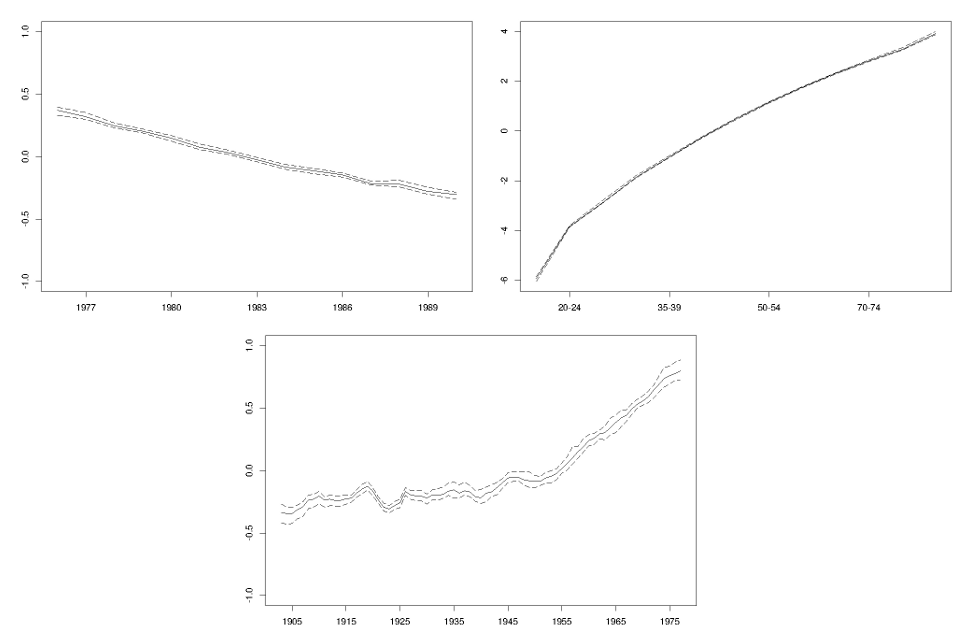
\includegraphics[scale=0.43]{../pics/sapc-apc.png}
\end{center}
\end{frame}
\begin{frame}
\begin{center}
\mode<presentation>{
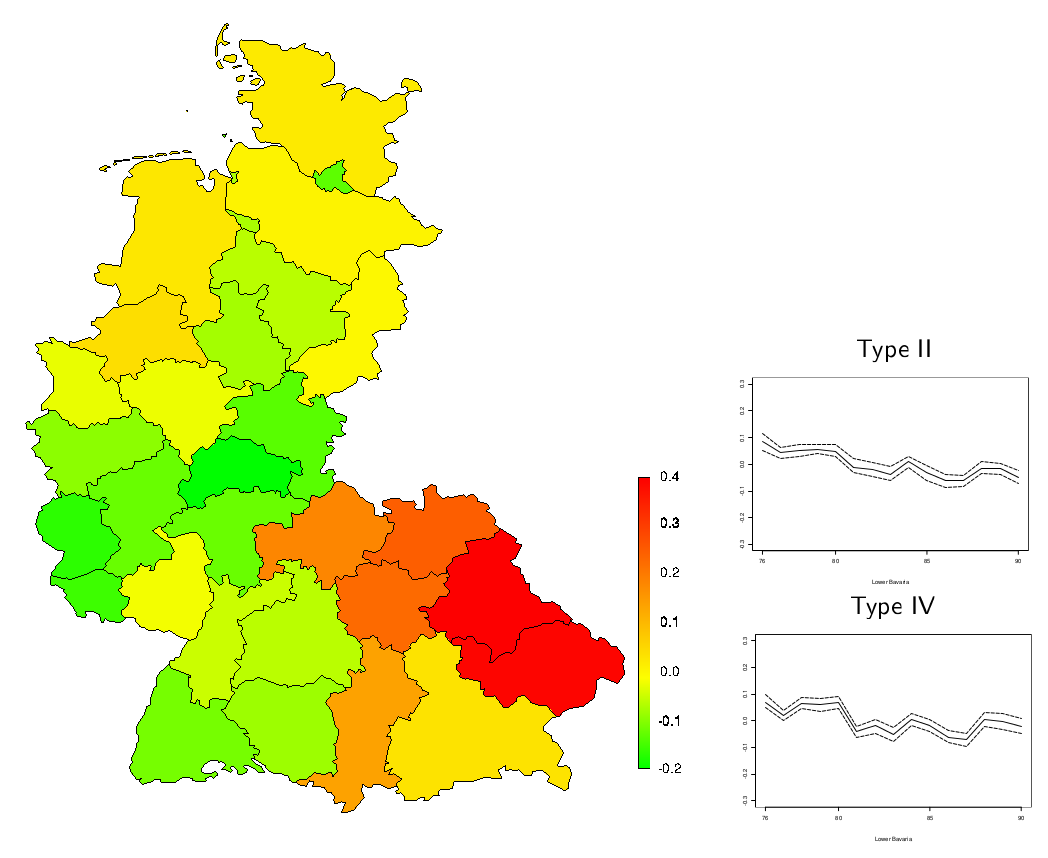
\includegraphics[scale=0.3]{../pics/sapc-interaktionen.png}
}
\mode<article>{
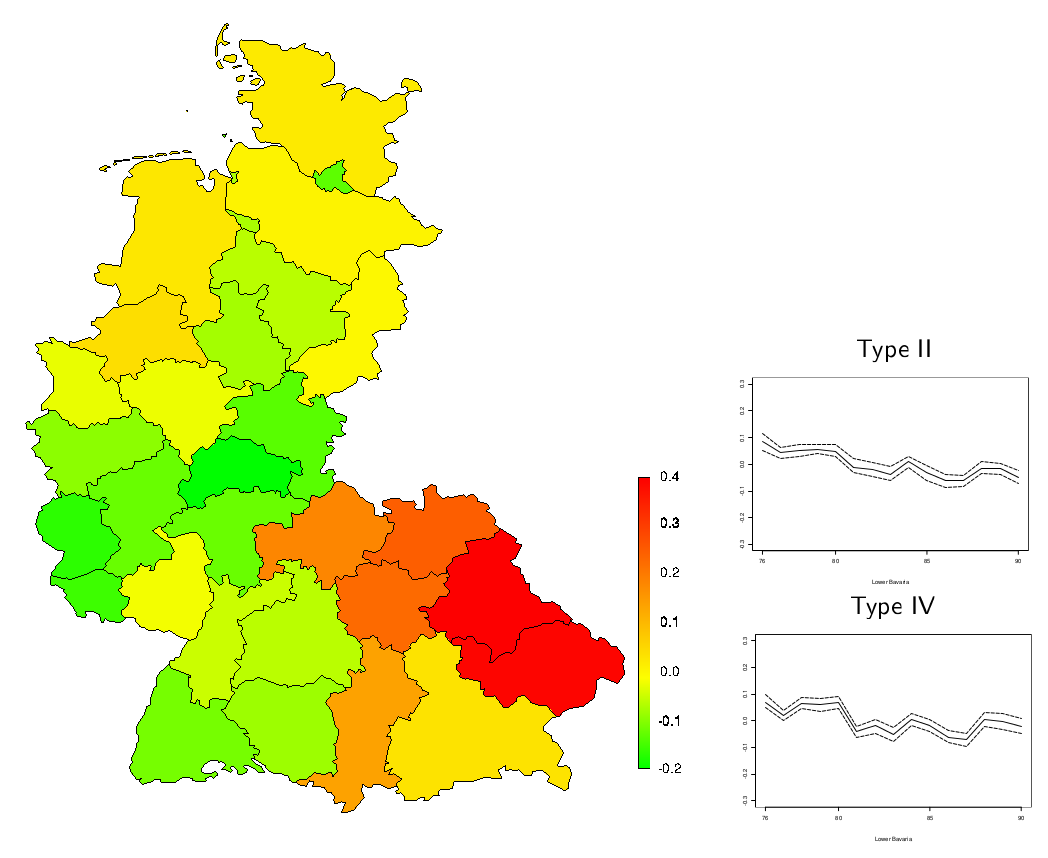
\includegraphics[scale=0.4]{../pics/sapc-interaktionen.png}
}
\end{center}
\end{frame}
\end{document}
